% Options for packages loaded elsewhere
\PassOptionsToPackage{unicode}{hyperref}
\PassOptionsToPackage{hyphens}{url}
%
\documentclass[
]{article}
\usepackage{amsmath,amssymb}
\usepackage{lmodern}
\usepackage{iftex}
\ifPDFTeX
  \usepackage[T1]{fontenc}
  \usepackage[utf8]{inputenc}
  \usepackage{textcomp} % provide euro and other symbols
\else % if luatex or xetex
  \usepackage{unicode-math}
  \defaultfontfeatures{Scale=MatchLowercase}
  \defaultfontfeatures[\rmfamily]{Ligatures=TeX,Scale=1}
\fi
% Use upquote if available, for straight quotes in verbatim environments
\IfFileExists{upquote.sty}{\usepackage{upquote}}{}
\IfFileExists{microtype.sty}{% use microtype if available
  \usepackage[]{microtype}
  \UseMicrotypeSet[protrusion]{basicmath} % disable protrusion for tt fonts
}{}
\makeatletter
\@ifundefined{KOMAClassName}{% if non-KOMA class
  \IfFileExists{parskip.sty}{%
    \usepackage{parskip}
  }{% else
    \setlength{\parindent}{0pt}
    \setlength{\parskip}{6pt plus 2pt minus 1pt}}
}{% if KOMA class
  \KOMAoptions{parskip=half}}
\makeatother
\usepackage{xcolor}
\IfFileExists{xurl.sty}{\usepackage{xurl}}{} % add URL line breaks if available
\IfFileExists{bookmark.sty}{\usepackage{bookmark}}{\usepackage{hyperref}}
\hypersetup{
  pdftitle={光线追踪:初步},
  pdfauthor={FlifeX, Red},
  hidelinks,
  pdfcreator={LaTeX via pandoc}}
\urlstyle{same} % disable monospaced font for URLs
\usepackage{graphicx}
\makeatletter
\def\maxwidth{\ifdim\Gin@nat@width>\linewidth\linewidth\else\Gin@nat@width\fi}
\def\maxheight{\ifdim\Gin@nat@height>\textheight\textheight\else\Gin@nat@height\fi}
\makeatother
% Scale images if necessary, so that they will not overflow the page
% margins by default, and it is still possible to overwrite the defaults
% using explicit options in \includegraphics[width, height, ...]{}
\setkeys{Gin}{width=\maxwidth,height=\maxheight,keepaspectratio}
% Set default figure placement to htbp
\makeatletter
\def\fps@figure{htbp}
\makeatother
\setlength{\emergencystretch}{3em} % prevent overfull lines
\providecommand{\tightlist}{%
  \setlength{\itemsep}{0pt}\setlength{\parskip}{0pt}}
\setcounter{secnumdepth}{-\maxdimen} % remove section numbering
\ifLuaTeX
  \usepackage{selnolig}  % disable illegal ligatures
\fi

\title{光线追踪:初步}
\author{FlifeX, Red}
\date{2021-06-05T22:05:00Z}

\begin{document}
\maketitle

\hypertarget{1-ux5f15ux8a00}{%
\subsection{1. 引言}\label{1-ux5f15ux8a00}}

\begin{quote}
本文需要一些关于向量的知识。
\end{quote}

时至今日,计算机图形学 (Computer Graphics, CG)
已经进入了生活的方方面面。这里不探讨 CG
技术对生活带来的影响,仅从它的基础出发,用 \texttt{Python} (没用到
\texttt{C++})来进行图形学的简要探讨。

本文所要实现的目标,是模拟极为简单的一个模型:一个\textbf{点光源}位于\textbf{平面}的正上方,求它发出的光(不考虑衰减------这涉及到光传播中的\textbf{平方反比定律})在该平面上各点的光强。

请注意:上文所提到的平面平行于电脑屏幕。这样,在这篇文章中,我们就可以减少坐标变换与映射的出现,也更好让初次接触
CG 的读者快速理解。

本文是系列文章的第一篇。作者本人也在同步学习。

\begin{itemize}
\item
  本文中所有渲染示意图均用 Blender 制作。
\end{itemize}

\hypertarget{2-ux56feux5f62ux5b66-hello-worldux5149}{%
\subsection{2. 图形学 Hello
World:光}\label{2-ux56feux5f62ux5b66-hello-worldux5149}}

这个小标题很好地说明了我们将要处理什么,以及它在整个图形学学习中的地位。先来介绍一些概念。

\hypertarget{21-ux5149ux7684ux53cdux5c04}{%
\subsubsection{2.1. 光的反射}\label{21-ux5149ux7684ux53cdux5c04}}

    

 图 1:光线的反射 

\textbf{定义 1.} 如\textbf{图 1},\(A\) 是任意一段光滑曲线。则,过 \(A\)
上一点作它的切线 \(t\) (tangent),再过交点 \(N\) 作 \(t\) 的垂线
\(n\),我们把直线 \(n\) 叫做曲线 \(A\) 在点 \(N\) 处的\textbf{法线}
(normal)。

\begin{center}\rule{0.5\linewidth}{0.5pt}\end{center}

再次看\textbf{图 1}。这一次我们注意打在曲线 \(A\)
上的那条线。如果这里把它看作光线,并把曲线 \(A\)
看作镜面,那么它叫做\textbf{入射光} (incident
ray)。自然,有入射光必定有\textbf{反射光} (reflected
ray),它和入射光关于法线 \(n\) 轴对称。图中的角 \(\theta\)
叫做\textbf{入射角} (incident angle),由上文我们可知\textbf{反射角}
(reflected angle) 在数值上等于入射角。

你可能已经感到疑惑:凭这些角,如何来刻画这束光照亮物体的程度呢?先暂时不看这幅图,接下来本文将一一介绍,光究竟如何照亮屏幕中的世界。

\hypertarget{211-ux5939ux89d2ux4e0eux660eux6697}{%
\paragraph{2.1.1. 夹角与明暗}\label{211-ux5939ux89d2ux4e0eux660eux6697}}

\begin{quote}
--- ``夹角''和``明暗''有什么关系?

--- 还真有。
\end{quote}

这里重申一下引言里的条件:不考虑光的衰减。现在,如果让你来刻画光线和平面夹角和平面上光所射中这一点的光照强度之间的关系,你会怎么做?请先思考,然后查看下面的折叠内容。

 一种解答 生活经验告诉我们,光在垂直照射某一样东西的时候,它将最亮。
(请不要想象手电筒或探照灯的光束------我们只是在谈论一丝光线,它没有体积。)
如果光线与物体的夹角是0度,则物体将不被照亮。
从0度到90度,从漆黑到明亮。你想到了哪个三角函数?
正是余弦函数。因此,计算出光和平面法向量的夹角余弦,便可以知道该点的明暗。
 

\hypertarget{22-ux5411ux91cfux5149ux7ebfux4e0eux5e73ux9762}{%
\subsubsection{2.2.
向量、光线与平面}\label{22-ux5411ux91cfux5149ux7ebfux4e0eux5e73ux9762}}

让我们顺着\textbf{2.1.1}中的思路,继续探究这个问题。

  

 图 2:点光源与平面 

如图,在空间中,我们可以把从点光源 \(L\)
发出的光线看作向量,并将它们反向,平移到光线与平面的接触点处,再计算平面上这一点的垂线所在的向量(我们把它叫做\textbf{法向量})与这束光的夹角的余弦。

你也许会注意到``接触点''一词。不过,这里完全可以选定一个点来计算,因为向量平移后仍等于原向量,这就是我们可以把所有向量平移到坐标原点简化运算的基础。

\begin{quote}
为什么不计算光线与平面的夹角?
\end{quote}

因为它们都是向量,所以可以考虑向量\textbf{点积} (dot
product)。一般来说,

\[\mathbf{a}\cdot\mathbf{b}=|\mathbf{a}||\mathbf{b}|\cos\langle\mathbf{a}, \mathbf{b}\rangle\]

这给了我们启示:两个向量之间的夹角,可以用它们的点积进行表达。但是,应该如何获取点积的值呢?下面,就引入用坐标表示点积的方法。

\textbf{定理.} 设
\(\mathbf{a}=(x_1, y_1, z_1)\),\(\mathbf{b}=(x_2, y_2, z_2)\),则它们的点积
\(\mathbf{a}\cdot\mathbf{b}\):

\[\mathbf{a}\cdot\mathbf{b}=x_1x_2+y_1y_2+z_1z_2\]

像这样,便可以由光线的坐标,得出光线和平面法向量之间的夹角的余弦值了。

此时会出现一个问题:从点光源 \(L\)
发出的光线是无穷多的。如果要每一束光线都涉及到,那么积分就必不可少。

但是,如果现在想象一张格点纸,只考虑击中在\textbf{格点上}的光线,并且只考虑\textbf{在纸上}的格点(也就是说平面不是无限大),那就可以用简单的离散运算来取得每一个选定点上的光强。

\hypertarget{221-ux8ba1ux7b97ux6570ux636e}{%
\paragraph{2.2.1 计算数据}\label{221-ux8ba1ux7b97ux6570ux636e}}

按上文所述的方法,我们便可以计算了。

在计算时要注意:光线向量是\textbf{可以变动}的,因为有无数条从无数个方向打到平面上的光,而平面(在我们的视角)只有一个法向量,因此需要把光线向量的坐标设为变量。

其次,就是炼丹学家喜闻乐见的\textbf{归一化}
(normalization)。这意味着要把所有向量转化为单位向量。实际上这很好办,直接用向量除以自己的\textbf{模}
(norm) 就行。

\textbf{定义 2}. 向量 \(\mathbf{v}\)
的模为根号下每个方向的坐标的平方之和,记作 \(|\mathbf{v}|\)。

然后再用光线向量和法向量的单位向量来计算夹角余弦:

\[\cos \theta = \frac{\frac{\mathbf{v_l}}{|\mathbf{v_l}|}\cdot\frac{\mathbf{n}}{|\mathbf{n}|}}{|\frac{\mathbf{v_l}}{|\mathbf{v_l}|}||\frac{\mathbf{n}}{|\mathbf{n}|}|}\]

\begin{center}\rule{0.5\linewidth}{0.5pt}\end{center}

\textbf{扩展阅读} 归一化的方法很多,包括但不限于 Sigmoid,softmax
等。但此处,直接把每个数据除以该组数据中的最大值即可。

\hypertarget{3-ux5f97ux5230ux7ed3ux679c}{%
\subsection{3. 得到结果}\label{3-ux5f97ux5230ux7ed3ux679c}}

\hypertarget{31-ux51c6ux5907}{%
\subsubsection{3.1. 准备}\label{31-ux51c6ux5907}}

理论上,像上面这样就可以了。但即使考虑的是平面且采样点有限,挨个手算也太复杂了。我们需要利用
\texttt{Python}。

\begin{figure}
\centering
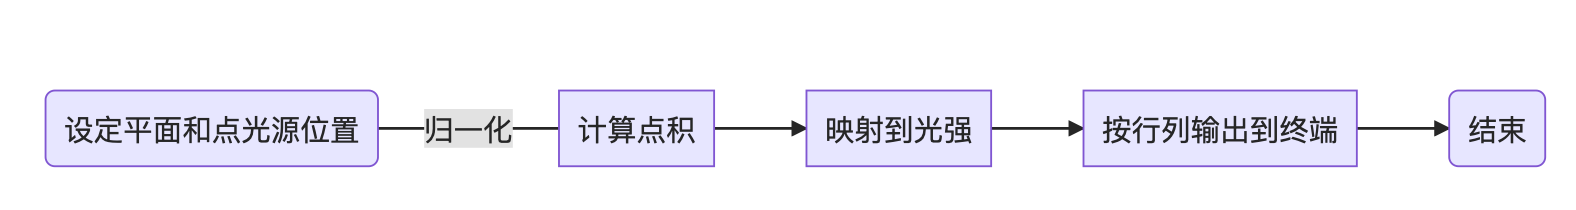
\includegraphics[width=8.20833in,height=\textheight]{image-20210722003504821.png}
\caption{}
\end{figure}

这样就需要向量来进行计算。由于 \texttt{Python}
不自带向量,所以必须写一个向量库。

\begin{verbatim}
|- venv
|  |- bin
|  |- lib
|  |  include
|  |  pyvenv.cfg
|
|  Float.py
|  Vector.py
|  main.py
\end{verbatim}

  树状图1:典型结构

其中,\texttt{Float.py} 和 \texttt{Vector.py} 都是所需的库,而
\texttt{main.py} 实现了流程图中的过程。

  

这是一个二维浮点数组类。它的 \texttt{magnitude()}
方法代表这个数组的模,因此可以用类似的思路,写一个三维浮点类,并用三维向量类来继承。这样,可以大大减少冗余代码量。

略去中间步骤,则最终可以得到:

  

不要乍一看被吓到了。实际上,真正起效的,只有 \texttt{\_\_mul\_\_()} 和
\texttt{ang()} 方法。前者是 \texttt{Python} 的魔术方法 (magic methods)
之一,允许用算符对两个对象进行运算操作。此处,"mul" 就是 multiply
的意思,方法内部重写的代码规定了两个向量如何相乘。

第 \texttt{22} 行,就是在 \textbf{2.2}
中提到过的夹角公式。同样,这个类也有 \texttt{normalized()}
方法来进行归一化处理。

\hypertarget{32-ux8ba1ux7b97}{%
\subsubsection{3.2. 计算}\label{32-ux8ba1ux7b97}}

  

这就是我们代码的核心,它通过计算夹角并一一映射到坐标点,提供了每个点的光强信息。

请注意其中第二行的注释。实际上并不需要定义光线向量,因为以击中点为参考系时,向量是可变的。因此我们可以直接在循环体内进行定义。

除此之外,9-12行的判断结构是为了把角度限制在0-90度内。但同样可以采用绝对值,这样会比判断快得多。

  

最后是 \texttt{Parse}
函数。它分为两部分,第一部分是把光强和字符一一映射,第二部分是将数据表示为可视化方阵。这就是用
\texttt{Python} 模拟光在平面上的照射情况的一个例子。

\hypertarget{33-ux793aux4f8b}{%
\subsubsection{3.3 示例}\label{33-ux793aux4f8b}}

\begin{enumerate}
\def\labelenumi{\arabic{enumi}.}
\item
  平面法向量 \((0, 0, 1)\), 点光源位置 \((0,0,0.1)\),大小
  \(35\times35\)。

    
\item
  平面法向量 \((3, 0, 1)\),其他条件不变。

    
\end{enumerate}

\hypertarget{4-ux603bux7ed3}{%
\subsubsection{4. 总结}\label{4-ux603bux7ed3}}

本文在图形学的基础上,使用 \texttt{Python}
对光线在平面上的光强进行了离散、简单的模拟。

下一篇文章将涉及到三维视图映射(相机视角)、曲面光强、光线衰减和漫反射,实际上是对此处介绍的
Lambert 光照模型的补全。以后还将介绍 Phong 光照模型和渲染方程,以及 BRDF
和 BSDF(双向反射、散射分布函数)。

感谢阅读。

\hypertarget{5-ux53c2ux8003}{%
\subsubsection{5. 参考}\label{5-ux53c2ux8003}}

\begin{quote}
这里的参考并不是指这篇文章参考了多少文献,而是提供一些扩展内容。
\end{quote}

\begin{enumerate}
\def\labelenumi{\arabic{enumi}.}
\item
  \href{https://benedikt-bitterli.me/tantalum/tantalum.html}{光路模拟}

  这是个非常棒的网站,而且作者在网站的博客内写的文章比我写的内容的水平高的多。强烈推荐。

  摘录其中几个极巧妙的公式:

  \[L_i(\mathbf{x}\leftarrow\vec{\omega})=L_o(t(\mathbf{x},\vec{\omega})\rightarrow-\vec{\omega}).\]

  \[L_o(\mathbf{x}\rightarrow\vec{\omega}_o)=L_e(\mathbf{x}\rightarrow\vec{\omega}_o)+\int_\Theta f(\vec{\omega}_i\rightarrow\vec{\omega}_o)L_i(\mathbf{x} \leftarrow\vec{\omega}_i)|\vec{\omega}_i\cdot N(\mathbf{x})|\mathrm{d}\vec{\omega}_i.\]

  \[\phi(\mathbf{x})=\int_{S^1}L_i(\mathbf{x}\leftarrow\vec{\omega})\mathrm{d}\vec{\omega}.\]

  \[\phi(\mathbf{x})\approx\sum_{i=1}^N\frac{L_o(t(\mathbf{x},-\vec{X}_i)\rightarrow\vec{X}_i))}{\operatorname{pdf}(\vec{X}_i)}.\]

  (不知道是 \(\KaTeX\) 还是 Hugo 的原因,只要公式内有 \texttt{aligned}
  环境或换行符,就无法正确渲染,只能分开替代。)
\end{enumerate}

\end{document}
